\section{ML based solution}

\subsection{Graph partitioning problem}

A graph neural network (GNN) is a deep learning paradigm that has gained a lot of popularity both in the deep learning and particle physics community in recent years \cite{I should find a few references for this}.

% Works that motivated me:
%\begin{itemize}
%\item The gnn formalism paper by Peter V
%\item Jonathan's b-tagging papers
%\item The Particle net bb tagger (maybe interaction networks too?)
%\item Trackig!
%\end{itemize}

To cast the 4b jet to parton assignment problem in the GNN formalism, consider and pp collision event as a graph where jets are the nodes of the graph, and a set of weighted connections.

The training objective becomes to maximize the edge weights between the jets that come from the same HC, as visualized in \Fig{\ref{fig:pag-partition}}.

\begin{figure}[hbt]
\centering
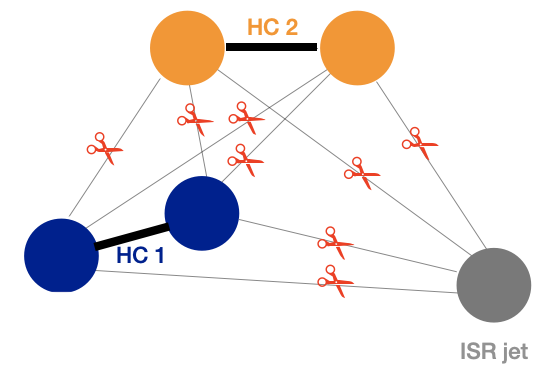
\includegraphics{figures/pairAGraph/pag-graph-partitioning}
\caption{}
\label{fig:pag-partition}
\end{figure}

Describe the space by a jet-similarity metric with similarity matrix $W$: 

\begin{equation}
	W_{ij} = \vec{j}_i \cdot \vec{j}_j
\end{equation}

Then for each event we can use this similarity matrix to define a \emph{score} for each possible pairing of jets into HCs. 

\textbf{\textcolor{hh:medturquoise}{Score:}} sum of similarity weights for pairing
\begin{itemize}
	\item HC1 formed from $\vec{j}_i$,  $\vec{j}_j$ 
	\item HC2 formed from $\vec{j}_k$,  $\vec{j}_l$ 
\end{itemize}

\begin{equation}
	\textcolor{hh:medturquoise}{s} = \vec{j}_i \cdot \vec{j}_j + \vec{j}_k \cdot \vec{j}_l
\end{equation}

\begin{figure}
	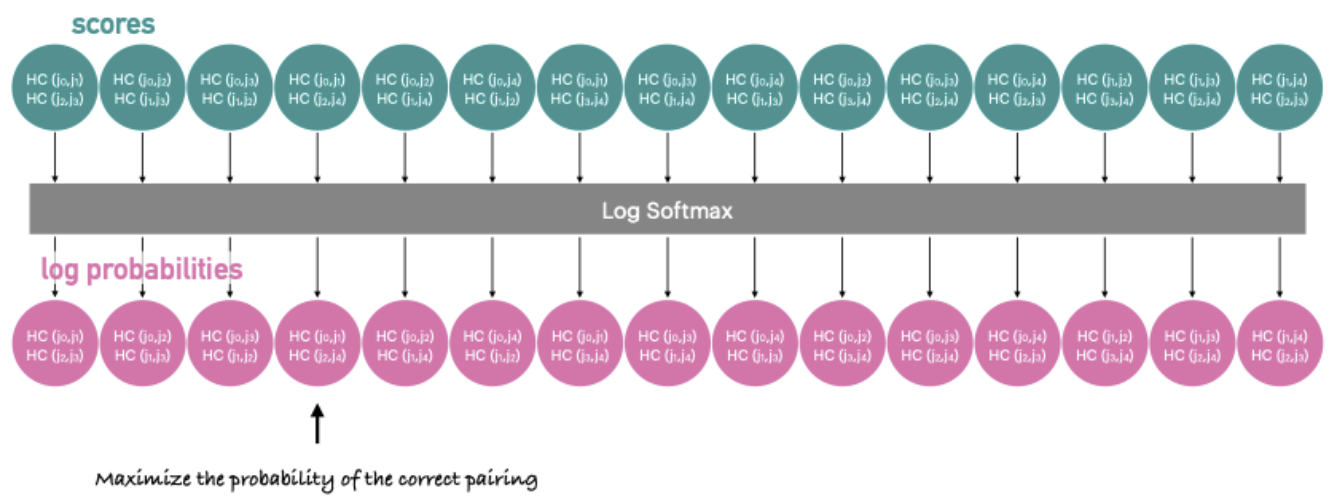
\includegraphics[width=\textwidth]{figures/pairAGraph/pag-loss}
	\caption{The loss function for a pairAGraph training event with 5 input jets.}
	\label{fig:pag-loss}
\end{figure}

\begin{figure}
	\centering
	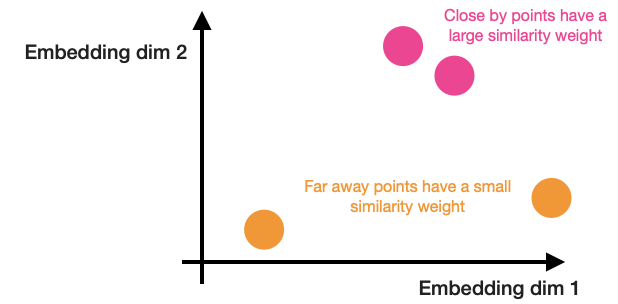
\includegraphics[width=.6 \textwidth]{figures/pairAGraph/embed-space}
	\caption{The jet embedding space.}
	\label{fig:embed-space}
\end{figure}


\subsection{Transformers}

The transformer architecture is now the state of the art in the natural language processing field for reasoning about the variable length sentences that we have today for large language models \hl{need GPT3 citation}.
The model was originally proposed for the task of neural machine translation \cite{1706.03762}, and used an encoder decoder architecture, as shown in \Fig{fig:xformer-fig1}.

\begin{figure}[hbt]
	\centering
	\subfloat{
		\label{fig:xformer-fig1}
		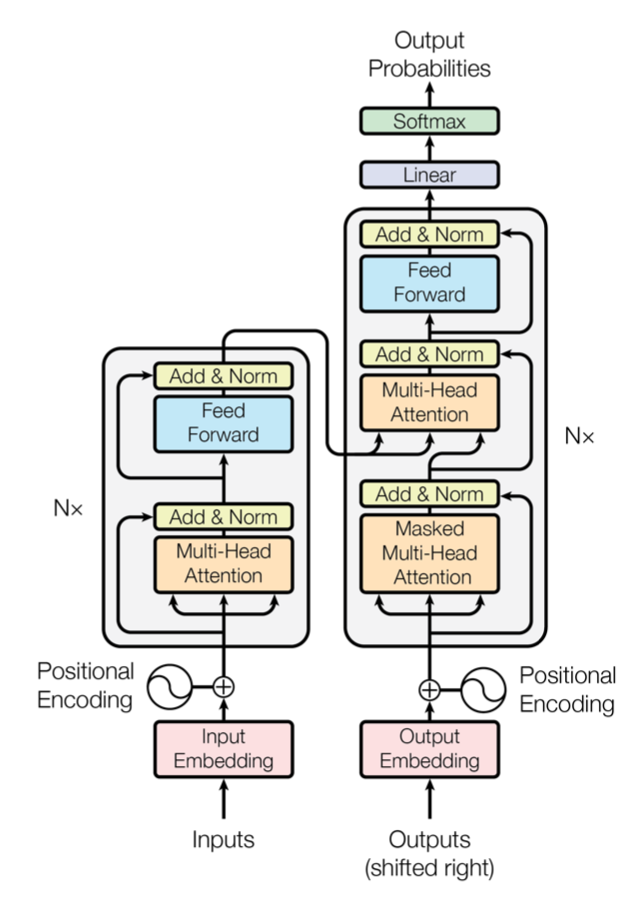
\includegraphics[width=.33\textwidth]{{figures/pairAGraph/xformer-fig1}}
	}
	\subfloat{
		\label{fig:xformer-fig2}
		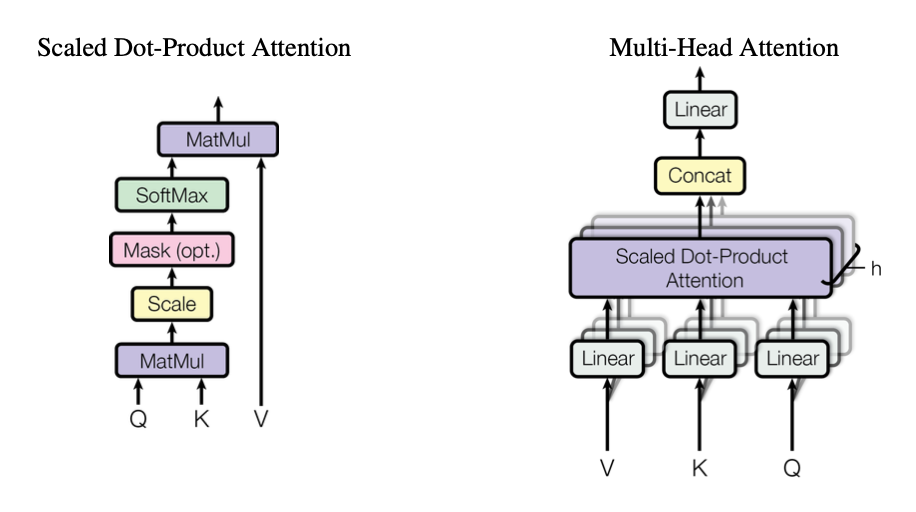
\includegraphics[width=.65\textwidth]{{figures/pairAGraph/xformer-fig2}}
	}
	\caption{The transformer architecture (left) and its building blocks: the weighted sum operation (middle) and the more expressive multi-head attention block formed by adding additional channels for the scaled dot product attention blocks (right) T \cite{1706.03762}.}
\end{figure}

Set transformer \cite{1810.00825}.

\FloatBarrier
\clearpage
\subsection{The 4b implementation: pairAGraph}

%\begin{itemize}
%\item \textbf{need to include the settings for the transformer training}
%\item Let's also say the number of training events that we used both for the SM and the kl = 10 training
%\item Also - I'm not sure if these results are with pre or post layer norm (I think pre, b/c I tried post in my next suite of opt studies, but it wasn't significantly better.)
%\end{itemize}

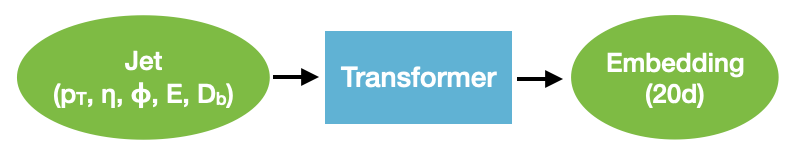
\includegraphics{figures/pairAGraph/pag-arch}

%I might want to check that this was the model that I was usig, but it looks like this might be it:
%{{xformer_1layers_dim20_ff20_4heads_dpt0.3_jetCompatibility_lr0.005_batch2048}}

Compared to the difficulty of the types of problems transformers are usually used for, this was quite a simple problem.
We used a small transformer model with only one of these ``multi-head attention'' blocks.
The jet latent dimension was 20, and  20 hidden units were used for computing the query and key weighted attention matrices. Four attention heads were used, and a dropout of rate of 0. 3 was applied to the nodes after the feed forward neural network layer. %We did a coarse hyperparameter
The loss was minimized with adam \cite{kingma2014adam} using a learning rate of 0.005 was a batch size of 2048 events. 
A validation set (20\% of the training events) were reserved for the training when the loss on this validation set hadn't improve in the last 20 epochs, and we took the model weights that had the best performance on the training dataset..

The training was done on events that passed the trigger and with at least 4 jets with \pt > 40 \GeV and two \Pqb-tags, and we combined events from the simulation corresponding to the 2016, 2017, and 2018 datasets. 


We used 2-fold cross validation training two transformers for each physics sample splitting the sample based on the event number.  
To evaluate the model with the even event numbers, we used the training that had been performed on the odd event numbers so that we could make full use of the final event statistics.

\subsection{Other baselines we compare to}

For my studies comparing the HC pairing accuracy, I compared to both the min dR algorithm (which was adopted in the 4b full Run 2 non-resonant analysis), and also to the baseline ``MDR+min($D_{hh}$)'' pairing.

\textbf{Briefly describe the MDR + min Dhh pairing}

\textbf{BDT pairing(?)}
